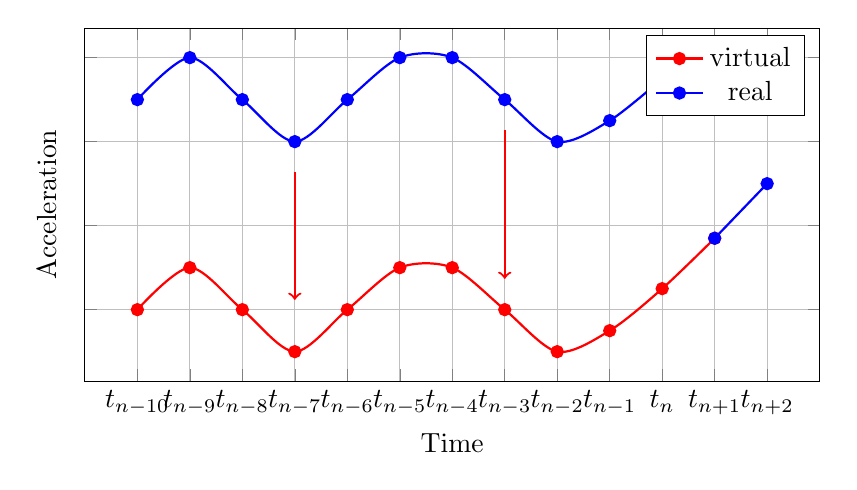
\begin{tikzpicture}[scale=1]

  \begin{axis}[
      height=0.5\textwidth,
      width=0.9\textwidth,
      xlabel = {Time},
      ylabel = {Acceleration},
      /pgf/number format/precision=10,
      xmin   = 0,
      xmax   = 14,
      %clip=false,
      %restrict x to domain=23:25,
      %x coord trafo/.code={\pgfmathparse{#1-5.0}\pgfmathresult} % x-offset MJD
      %ymin   = 0,
      %ymax   = 0.01,
      xtick  = {1,2,3,4,5,6,7,8,9,10,11,12,13,14},
      %ytick  = {},
      %minor x tick num={1},
      %minor y tick num={3},
      scaled ticks = true,
      ymajorgrids,
      yminorgrids,
      xmajorgrids,
      xminorgrids,
      yticklabels={,,},
      xticklabels={$t_{n-10}$,$t_{n-9}$,$t_{n-8}$,$t_{n-7}$,$t_{n-6}$,$t_{n-5}$,$t_{n-4}$,$t_{n-3}$,$t_{n-2}$,$t_{n-1}$,$t_{n}$,$t_{n+1}$,$t_{n+2}$},
      legend entries={virtual, real} ,
      %legend style={at={(0.02,0.98)}, anchor=north west},
      %legend cell align = left
      %every y tick label/.append style  =
       % { 
        %  /pgf/number format/.cd,
         %  precision = 3, 
          % fixed
        %}
  ]
    
    \addplot[red,thick,mark=*,smooth]  coordinates {(1,15-5)(2,16-5)(3,15-5)(4,14-5)(5,15-5)(6,16-5)(7,16-5)(8,15-5)(9,14-5)(10,14.5-5)(11,15.5-5)(12,16.7-5)};
    
    \addplot[blue,thick,mark=*,smooth]  coordinates {(1,15)(2,16)(3,15)(4,14)(5,15)(6,16)(7,16)(8,15)(9,14)(10,14.5)(11,15.5)
    
                                                     (12,16.7-5)(13,18-5)};
                                                     
    \node (source1)      at   ( axis cs: 4,13.5 ){};
    \node (destination1) at   ( axis cs: 4,10   ){};
    
    \node (source2)      at   ( axis cs: 8,14.5 ){};
    \node (destination2) at   ( axis cs: 8,10.5 ){};
    
    \draw[->,thick,red](source1)--(destination1);
    \draw[->,thick,red](source2)--(destination2);
    
    %\node (c1) at (axis cs:2,0.224309) {$\cdot 10^{-3}$};
  \end{axis}
  
\end{tikzpicture}